\documentclass[10pt]{article}
\usepackage[utf8]{inputenc}
\usepackage[T1]{fontenc}
\usepackage{amsmath}
\usepackage[spanish]{babel}
\usepackage{amsfonts}
\usepackage{amssymb}
\usepackage{mhchem}
\usepackage{stmaryrd}
\usepackage{graphicx}
\usepackage[export]{adjustbox}
\graphicspath{ {./images/} }
\usepackage{bbold}


\title {\textbf{Un algoritmo de dos fases para reconocer actividades humanas en el contexto de la Industria 4.0 y los procesos impulsados por el ser humano }}


\author{Borja Bordel $^{1}$, Ramón Alcarria ${ }^{1}$, Diego Sánchez-de-Rivera ${ }^{1}$\\
${ }^{1}$ Universidad Politécnica de Madrid,\\
Madrid, España\\
bbordel@dit.upm.es, ramon.alcarria@upm.es,diegosanchez@dit.upm.es}
\date{}


\begin{document}
\maketitle


\begin{abstract}
 Los futuros sistemas industriales, una revolución conocida como Industria 4.0, están previstos para integrar a las personas en el mundo cibernético como prosumidores (proveedores de servicios y consumidores). En este contexto, los procesos impulsados por humanos aparecen como una realidad esencial y se requieren instrumentos para crear bucles de información de retroalimentación entre el subsistema social (personas) y el subsistema cibernético (componentes tecnológicos). Aunque se han propuesto muchos instrumentos diferentes, hoy en día las técnicas de reconocimiento de patrones son las más prometedoras. Sin embargo, estas soluciones presentan algunos problemas pendientes importantes. Por ejemplo, dependen del hardware seleccionado para adquirir información de los usuarios; o presentan un límite en la precisión del proceso de reconocimiento. Para abordar esta situación, en este trabajo se propone un algoritmo de dos fases para integrar personas en la Industria 4. 0 sistemas y procesos impulsados por humanos. El algoritmo define acciones complejas como composiciones de movimientos simples. Las acciones complejas se reconocen utilizando modelos ocultos de Markov y los movimientos simples se reconocen utilizando Dynamic Time Warping. De esa manera, solo los movimientos dependen de los dispositivos de hardware empleados para capturar información, y la precisión del reconocimiento de acciones complejas aumenta considerablemente. También se realiza una validación experimental real para evaluar y comparar el rendimiento de la solución propuesta. y la precisión del reconocimiento de acciones complejas aumenta considerablemente. También se realiza una validación experimental real para evaluar y comparar el rendimiento de la solución propuesta. y la precisión del reconocimiento de acciones complejas aumenta considerablemente. También se realiza una validación experimental real para evaluar y comparar el rendimiento de la solución propuesta. 

\end{abstract}

Palabras clave: Industria 4.0; reconocimiento de patrones; Dynamic Time Warping; Inteligencia artificial; Modelos ocultos de Markov.

\section{Introducción}
La Industria 4.0 [1] se refiere al uso de Sistemas Ciber-Físicos (uniones de procesos físicos y cibernéticos) [2] como componente tecnológico principal en futuras soluciones digitales, principalmente (pero no solo) en escenarios industriales. Típicamente, la digitalización ha provocado, al final, la sustitución de los mecanismos tradicionales de trabajo por nuevos instrumentos digitales. Por ejemplo, los trabajadores de las cadenas de montaje fueron sustituidos por robots durante la tercera revolución industrial. Sin embargo, algunas aplicaciones industriales no pueden basarse en soluciones tecnológicas, siendo aún imprescindible el trabajo humano [3]. Los productos hechos a mano son un ejemplo de aplicaciones donde la presencia de obras humanas es fundamental. Estos sectores industriales, en cualquier caso, también deben integrarse en la cuarta revolución industrial. De la unión de Traducido del inglés al español. Los Sistemas Ciber-Físicos (CPS) y los humanos actuando como proveedores de servicios (obras activas), surgen los CPS humanizados [4]. En estos nuevos sistemas, se permiten procesos impulsados por humanos [5]; es decir, procesos que son conocidos, ejecutados y gestionados por personas (aunque pueden estar vigilados por mecanismos digitales). Para crear una integración real entre las personas y la tecnología, y mover la ejecución del proceso desde el subsistema social (humanos) al mundo cibernético (componentes de hardware y software), se necesitan técnicas para la extracción de información. Se han reportado muchas soluciones y enfoques diferentes durante los últimos años, pero hoy en día las técnicas de reconocimiento de patrones son las más prometedoras. El uso de Inteligencia Artificial, modelos estadísticos y otros instrumentos similares han permitido un desarrollo real e increíble de soluciones de reconocimiento de patrones, pero aún quedan algunos retos pendientes. En primer lugar, las técnicas de reconocimiento de patrones dependen del dispositivo de hardware subyacente para la captura de información. La estructura y el proceso de aprendizaje cambia si (por ejemplo) en lugar de acelerómetros consideramos sensores infrarrojos. Esto es muy problemático ya que las tecnologías de hardware evolucionan mucho más rápido que las soluciones de software. Y, segundo, hay un límite a la precisión en el proceso de reconocimiento. De hecho, a medida que las acciones humanas se vuelven más complicadas, se requieren más variables y modelos más complejos para reconocerlas. Este enfoque genera grandes problemas de optimización cuyo error residual es mayor a medida que aumenta el número de variables; lo que provoca una disminución en la tasa de reconocimiento de éxito [6]. En conclusión, las matemáticas (no el software, por lo tanto, no depende de la implementación) obligan a una cierta precisión para el proceso de reconocimiento de patrones dadas las acciones a estudiar. Para evitar esta situación, se debe considerar un menor número de variables, pero esto también reduce la complejidad de las acciones que se pueden analizar; una solución que no es aceptable en escenarios industriales donde se desarrollan actividades productivas complejas. Por lo tanto, el objetivo de este artículo es describir un nuevo algoritmo de reconocimiento de patrones que aborde estos dos problemas básicos. El mecanismo propuesto define las acciones como una composición de movimientos simples. Los movimientos simples se reconocen mediante técnicas de deformación dinámica del tiempo (DTW) [7]. Este proceso depende del hardware seleccionado para la captura de información; pero los DTW son muy flexibles y actualizar el repositorio de patrones es suficiente para reconfigurar todo el algoritmo. Luego, las acciones complejas se reconocen como combinaciones de movimientos simples a través de los Modelos Ocultos de Markov (HMM) [8]. Estos modelos son totalmente independientes de las tecnologías de hardware, ya que solo consideran acciones simples. Este enfoque de dos fases también reduce la complejidad de los modelos, aumentando la precisión y la tasa de éxito en el proceso de reconocimiento. El resto del documento está organizado de la siguiente manera: la Sección 2 describe el estado del arte sobre el reconocimiento de patrones para las actividades humanas; la Sección 3 describe la solución propuesta, incluyendo las dos fases definidas; la sección 4 presenta una validación experimental utilizando un escenario real y usuarios finales; y la Sección 5 concluye el documento. 


\section{Reconocimiento de patrones de vanguardia }

Se han informado muchas técnicas diferentes de reconocimiento de patrones para actividades humanas. Sin embargo, la propuesta más común puede clasificarse en cinco categorías [9]: (i) Modelos ocultos de Markov; (ii) el campo aleatorio condicional de cadena de salto; (iii) Patrones Emergentes; (iv) el Campo Aleatorio Condicional; y (v) clasificadores bayesianos. De hecho, la mayoría de los autores proponen el uso de Modelos Ocultos de Markov (HMM) para modelar las actividades humanas. HMM permite modelar acciones como cadenas de Markov [10][11]. Básicamente, HMM genera estados ocultos a partir de datos observables. En particular, el objetivo final de esta técnica es construir la secuencia de estados ocultos que encaje con una determinada secuencia de datos. Para finalmente definir todo el modelo, HMM debe deducir de los datos los parámetros del modelo de manera confiable. La figura 1 muestra una representación esquemática de cómo funciona HMM. Cuando se reconocen las actividades humanas, las acciones que componen las actividades son los estados ocultos y las salidas de los sensores son los datos que se estudian. HMM, además, permite el uso de técnicas de entrenamiento considerando el conocimiento previo sobre el modelo. Este entrenamiento a veces es esencial para “inducir” todas las posibles secuencias de datos requeridas para calcular el HMM. Por último, es muy importante señalar que los HMM aislados simples se pueden combinar para crear modelos más grandes y complejos.


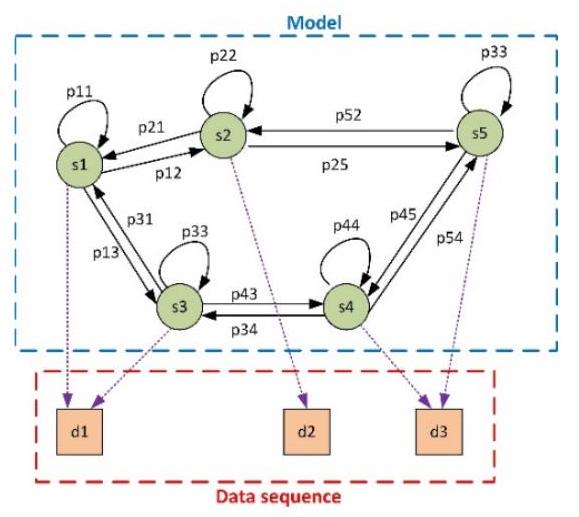
\includegraphics[max width=\textwidth]{2022_09_15_69d89c46b49bb93649d1g-03}

Fig. 1. Representación gráfica de un HMM\\

Los HMM, sin embargo, son inútiles para modelar ciertas actividades concurrentes, por lo que otros autores han reportado una nueva técnica denominada Conditional Random Field (CRF). Los CRF se emplean para modelar aquellas actividades que presentan acciones concurrentes o, en general, múltiples acciones que interactúan [12][13]. Además, HMM requiere un gran esfuerzo de entrenamiento para descubrir todos los estados ocultos posibles. Para resolver estos problemas, el campo aleatorio condicional (CRF) emplea probabilidades condicionales en lugar de distribuciones de probabilidad conjunta. De esa forma, se pueden modelar fácilmente actividades cuyas acciones se desarrollan en cualquier orden. A diferencia de las cadenas en HMM, CRF emplea gráficos acíclicos y permite la integración de estados ocultos condicionales (estados que dependen de observaciones pasadas y/o futuras). Los CRF, por otro lado, siguen siendo inútiles para modelar ciertos comportamientos, por lo que algunas propuestas generalizan este concepto y proponen el Skip Chain Conditional Random Field (SCCRF). SCCRF es una técnica de reconocimiento de patrones, más general que CRF, que permite modelar actividades que no son una secuencia de acciones en la naturaleza [14]. Esta técnica trata de capturar dependencias de largo alcance (cadena de salto); y puede entenderse como el producto de diferentes cadenas lineales. Sin embargo, calcular este producto es bastante pesado y complicado, por lo que esta técnica suele ser demasiado costosa desde el punto de vista computacional para implementarla en pequeños sistemas integrados. Otras propuestas emplean técnicas de descripción de mayor nivel como Emerging Patterns (EP). Para la mayoría de los autores, EP es una técnica que describe actividades como vectores de parámetros y sus valores correspondientes (ubicación, objeto, etc.) [15]. Utilizando distancias entre vectores es posible calcular y reconocer acciones desarrolladas por personas. Finalmente, otros autores han empleado con éxito técnicas secundarias como los clasificadores bayesianos [16], que identifican actividades haciendo una correspondencia entre las actividades humanas y las salidas más probables de los sensores mientras se realizan estas acciones, considerando que todos los sensores son independientes. Los árboles de decisión [17], las extensiones HMM [18] y otras tecnologías similares también se han estudiado en la literatura, aunque estas propuestas son escasas. Entre todas las tecnologías descritas, HMM no es la más poderosa. Sin embargo, encaja a la perfección con la Industria 4.0, donde las actuaciones son muy complejas pero muy estructuradas y ordenadas (según protocolos de empresa, políticas de eficiencia, etc.). Además, se requiere una retroalimentación rápida (a veces incluso en tiempo real) para garantizar que los procesos impulsados por humanos funcionen correctamente antes de que ocurra una falla crítica global. Por lo tanto, las soluciones computacionalmente costosas no son un enfoque válido, y estamos seleccionando HMM como tecnología de base principal. Para preservar su carácter liviano y, al mismo tiempo, poder modelar actividades complejas, introducimos un esquema de reconocimiento de dos fases que permite dividir acciones complejas en dos pasos más simples. 


\section{Un algoritmo de reconocimiento de patrones de dos fases}
Con el fin de (i) independizar el proceso de reconocimiento de patrones de los dispositivos de
hardware empleados para capturar información, (ii) permitir el reconocimiento de acciones
complejas y (iii) preservar el carácter liviano de los modelos seleccionados, la solución propuesta
presenta una arquitectura con tres capas diferentes (ver Figura 2).

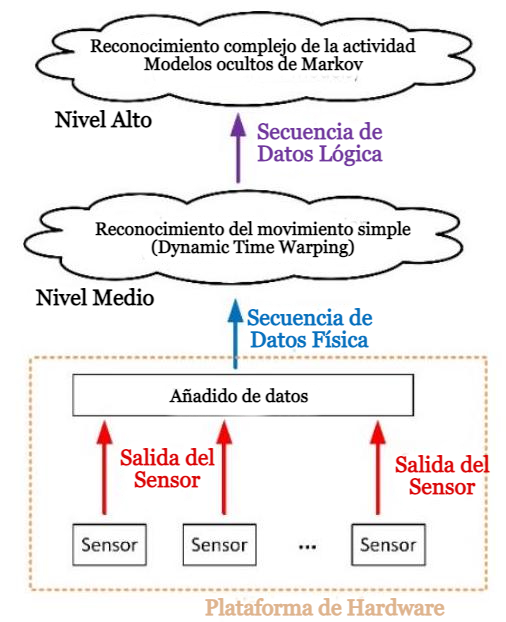
\includegraphics[max width=\textwidth]{2022_09_15_69d89c46b49bb93649d1g-04}

Fig. 2. Arquitectura de la solución de reconocimiento de patrones propuesta 

La capa más baja incluye la plataforma de hardware. Los dispositivos de monitoreo como acelerómetros, teléfonos inteligentes, sensores infrarrojos, etiquetas RFID, etc., se implementan para capturar información sobre el comportamiento de las personas. Las salidas de estos dispositivos crean secuencias de datos físicos cuyo formato, rango dinámico, etc., dependen totalmente de las tecnologías de hardware seleccionadas. Estas secuencias de datos físicos luego se procesan en la capa intermedia utilizando técnicas DTW. Como resultado, para cada secuencia de datos físicos, se reconoce un movimiento o acción simple. Estas acciones simples se representan mediante un formato de datos binarios para que la solución sea lo más ligera posible. El software en este nivel debe modificarse cada vez que se actualiza la plataforma de hardware, pero las tecnologías DTW no requieren un proceso de actualización pesado, y actualizar el repositorio de patrones es suficiente para configurar el algoritmo en este nivel. Los movimientos simples reconocidos, entonces, se agrupan para crear secuencias de datos lógicos. Estas secuencias alimentan un sistema de reconocimiento de patrones de alto nivel basado en modelos ocultos de Markov. En este nivel, los componentes de software requieren un proceso de entrenamiento pesado, pero la capa intermedia hace que la plataforma de hardware y los modelos de alto nivel sean totalmente independientes. Por lo tanto, cualquier cambio en la plataforma de hardware no impone una actualización en el HMM, lo que sería extremadamente costoso desde el punto de vista computacional. Mediante el análisis de la secuencia de movimientos simples, se reconocen acciones complejas. La siguiente subsección describe en detalle las dos fases de reconocimiento de patrones propuestas.

\subsection{Reconocimiento de movimiento simple: Dynamic Time Warping}
Para reconocer gestos o movimientos simples, se selecciona una solución Dynamic Time Warping. Las tecnologías DTW cumplen con los requisitos de los componentes de software de nivel medio, ya que se adaptan muy fácilmente a las características de la plataforma de hardware subyacente y son bastante rápidas y eficientes (por lo que los pequeños dispositivos integrados pueden implementarlas). En nuestra solución, el comportamiento humano es monitoreado a través de una familia de sensores , que contiene componentes (1). 

$$
\mathcal{S}=\left\{s_{i}, i=1, \ldots, N_{s}\right\}
$$
Las salidas de estos sensores se muestrean periódicamente cada    segundos; obteniendo para cada instante de tiempo,  ,un vector de    (cada valor de cada sensor). este vector    se llama “una muestra multidimensional”. (2) 
$$
Y_{t}=\left\{y_{t}^{i}, i=1, \ldots, N_{s}\right\}
$$
Entonces, un simple movimiento  tendrá una duración de    segundos y será descrita por la secuencia temporal de    muestras multidimensionales recolectadas durante este tiempo (3). Para reconocer posteriormente los movimientos, un repositorio de patronesℛse crea conteniendo las correspondientes secuencias temporales para cada uno de los  acciones simples para ser reconocidas (4)
$$
\begin{gathered}
Y=\left\{Y_{t}, t=1, \ldots, T_{m}\right\}=\left\{Y^{i}, i=1, \ldots, N_{m}\right\} \\
\mathcal{R}=\left\{R_{i}, i=1, \ldots, K\right\}
\end{gathered}
$$
En general, las personas realizan movimientos de manera similar pero diferente. Así, las transiciones pueden ser más lentas o más rápidas, se pueden agregar o quitar algunas acciones elementales, etc.  Por lo tanto, dada una secuencia $X$ con $N_{x}$ muestras, representando un movimiento a ser reconocido, se debe localizar el $R_{i} \in \mathcal{R}$ más cerca a $X$; así que $R_{i}$ se reconoce como la acción realizada. Para ello se define una función distancia (5). Esta función de distancia se puede aplicar para calcular una matriz de costos, requerida ya que las muestras generalmente no tienen la misma longitud ni están alineadas (6).